\documentclass[12pt,a4paper]{article}
\usepackage{amsmath}
\usepackage[english]{babel}
\usepackage{graphicx}
\usepackage{listings}
\usepackage{fullpage}
\usepackage[T1]{fontenc}
\usepackage{enumerate}
\usepackage[makeroom]{cancel}
\usepackage{hyperref}

\lstdefinestyle{custompython}{
  belowcaptionskip=1\baselineskip,
  breaklines=true,
  frame=L,
  xleftmargin=\parindent,
  language=bash,
  basicstyle=\footnotesize\ttfamily,
  showstringspaces=false,
  %commentstyle=\itshape\color{purple!40!black},
  %keywordstyle=\itshape\color{green!40!black},
  %identifierstyle=\color{blue},
  %stringstyle=\color{orange},
}

\author{
  Cheng, Lidens\\
  \texttt{lidenscheng@email.arizona.edu}
  \and
  McClintock, Tom\\
  \texttt{tmcclintock@email.arizona.edu}
  \and
  Wagoner, Erika\\
  \texttt{wagoner47@email.arizona.edu}
}
\title{Astr 513: Homework 2}

\begin{document}
\maketitle
  
\section{Parts A and B}

\begin{enumerate}[a)]
 \item We can use three kinematic equations to find $u_x$ and $u_y$ in terms of $R$, $g$, and $h$:
 \begin{enumerate}[(1)]
  \item $0 = u_y^2 - 2 g h \Rightarrow \boxed{u_y = \sqrt{2 g h}}$
  \item $0 = u_y - \frac{g t}{2} = \sqrt{2 g h} - \frac{g t}{2} \Rightarrow t = \sqrt{\frac{8 h}{g}}$
  \item $R = u_x t = u_x \sqrt{\frac{8 h}{6}} \Rightarrow \boxed{u_x = R \sqrt{\frac{g}{8h}}}$
 \end{enumerate}
 In the error propagation method, the expected values for $u_x$ and $u_y$ are just the values $u_x^0$ and $u_y^0$ we obtain when we insert the mean values $R_0$, $g_0$, and $h_0$ into the expressions above:
 \begin{subequations}
  \begin{align*}
   u_x^0 &= R_0 \sqrt{\frac{g}{8 h}} \\
   &= 10.0 \mathrm{m} \sqrt{\frac{9.81 \cancel{\mathrm{m}} \cdot \mathrm{s}^{-2}}{8 \cdot 1.0 \cancel{\mathrm{m}}}}
  \end{align*}
  \begin{equation}
   \boxed{u_x^0 \approx 11.1 \mathrm{m} \cdot \mathrm{s}^{-1}}
  \end{equation}
 \end{subequations}
 \begin{subequations}
  \begin{align*}
   u_y^0 &= \sqrt{2 g_0 h_0} \\
   &= \sqrt{2 \cdot 9.81 \mathrm{m} \cdot \mathrm{s}^{-2} \cdot 1.0 \mathrm{m}}
  \end{align*}
  \begin{equation}
   \boxed{u_y^0 \approx 4.43 \mathrm{m} \cdot \mathrm{s}^{-1}}
  \end{equation}
 \end{subequations}
 
 When using propagation of errors, the fractional error on some function $f\left(\vec{x}\right)$ with mean $\vec{x}$ values $\vec{x}^0$ and errors $\sigma_i$ can be found by $\frac{\sigma_f}{f} = \sqrt{\displaystyle \sum_{i = 1}^n \left(\frac{\partial \ln f}{\partial x_i}\right)_{\vec{x}^0} \sigma_i^2 }$. So we first take the natural log of $u_x$ and $u_y$:
 \begin{align*}
  \ln u_x &= \ln R + \frac{1}{2} \ln g - \frac{1}{2} \ln h - \frac{3}{2} \ln 2 \\
  \ln u_y &= \ln 2 + \ln g + \ln h
 \end{align*}
 Then we find that
 \begin{subequations}
  \begin{align*}
   \frac{\sigma_{u_x}}{u_x} &= \sqrt{\left(\frac{\sigma_R}{R_0}\right)^2 + \frac{1}{4} \left(\frac{\sigma_g}{g_0}\right)^2 + \frac{1}{4} \left(\frac{\sigma_h}{h_0}\right)^2} \\
   &= \sqrt{\left(\frac{0.2\cancel{\mathrm{m}}}{10.0\cancel{\mathrm{m}}}\right)^2 + \frac{1}{4} \left(\frac{0.05 \cancel{\mathrm{m}} \cdot \cancel{\mathrm{s}^{-2}}}{9.81 \cancel{\mathrm{m}} \cdot \cancel{\mathrm{s}^{-2}}}\right)^2 + \frac{1}{4} \left(\frac{0.2 \cancel{\mathrm{m}}}{1.0 \cancel{\mathrm{m}}}\right)^2}
  \end{align*}
  \begin{equation}
   \boxed{\frac{\sigma_{u_x}}{u_x} \approx 0.10}
  \end{equation}
 \end{subequations}
 for $\sigma_{u_x}$, and for $\sigma_{u_y}$,
 \begin{subequations}
  \begin{align*}
   \frac{\sigma_{u_y}}{u_y} &= \sqrt{\frac{1}{4} \left(\frac{\sigma_g}{g_0}\right)^2 + \frac{1}{4} \left(\frac{\sigma_h}{h_0}\right)^2} \\
   &= \frac{1}{2} \sqrt{\left(\frac{0.05 \cancel{\mathrm{m}} \cdot \cancel{\mathrm{s}^{-2}}}{9.81 \cancel{\mathrm{m}} \cdot \cancel{\mathrm{s}^{-2}}}\right)^2 + \left(\frac{0.2 \cancel{\mathrm{m}}}{1.0 \cancel{\mathrm{m}}}\right)^2}
  \end{align*}
  \begin{equation}
   \boxed{\frac{\sigma_{u_y}}{u_y} \approx 0.10}
  \end{equation}
 \end{subequations}
 
 \item Now we use Monte Carlo realizations of $R$, $g$, and $h$ assuming Gaussian uncertainties to find the distributions of $u_x$ and $u_y$. Using this method, we find that $u_x \approx 11.1\substack{+1.32 \\ -0.99}$ and $u_y \approx 4.43\substack{+0.42 \\ -0.46}$. So the means for $u_x$ and $u_y$ seem to agree with the error propagation method, but not the errors. The marginalized distributions for $u_x$ and $u_y$, as well as the distribution of $u_y$ vs $u_x$, can be seen in the corner plot in Fig ~\ref{fig:2.1b}.
 
 \begin{figure}[ht]
  \centering
  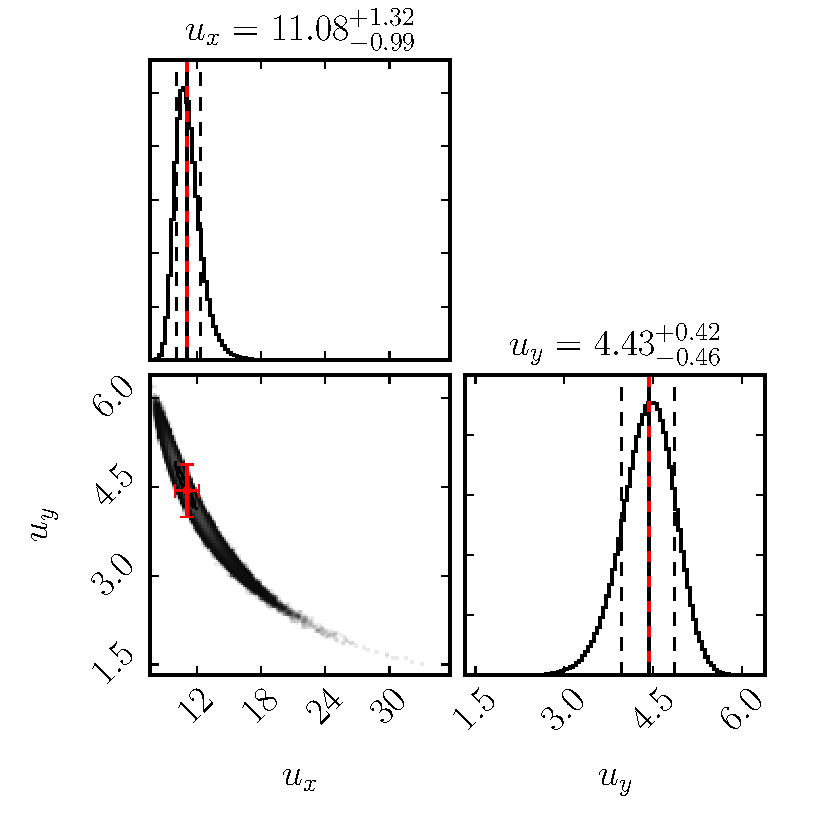
\includegraphics[keepaspectratio]{hw2_b_corner.pdf}
  \caption{The distribution of $u_y$ vs $u_x$ as well as the marginalized distributions for $u_x$ and $u_y$. The red line in the marginalized distributions shows the answer from the error propagation method, and the red point with error bars is the expected value and error from the error propagation method.}
  \label{fig:2.1b}
 \end{figure}
\end{enumerate}

\section{Part C}

\section{Part D}
Bayes' Theorem says
\begin{equation}
  P(A|B) = \frac{P(B|A)P(A)}{P(B)}
\end{equation}
where $P(X|Y)$ is a conditional probability of $X$ given $Y$, and $P(Z)$ is 
refered to as a \textit{prior} belief on what the value of $Z$ should be.
Frequentists equate the two conditional probabilities, but this is incorrect
in the Bayesian approach precisely because you wish to be informed by the 
priors. In this part, we assume \textit{uniform} priors on our posterior
parameters $u_x$, $u_y$ and $g$, and in addition to this there is no Jacobian 
transformation. Thus we can write for the conditional probability
\begin{equation}

\end{equation}

\newpage

\section*{References}

\end{document}
